\section{Durchführung}

    In diesem Versuch werden Fehlstellen in einem Plexiglasquader lokalisiert
    und die Abstände in einem Augemodell gemessen.\\
    \\
    Für die Messung stehen ein Ultraschallechoskop,
    eine Ultraschallsonde mit einer Frequenz von $\SI{2}{\mega\hertz}$ und ein Computer mit einem Messprogramm zur Verfügung.
    Das Programm verfügt über die Einstellung der Laufzeit- und Tiefenmessung,
    wobei in diesem Versuch die Laufzeiten der Schallimpulse und die zugehörigen Spannungsamplituden gemessen werden.
    Mit einem Curser können die Peaks der Spannung,
    welche bei Fehlstellen in der Probe entstehen,
    genau gemessen werden,
    wobei hier das Impuls-Echo-Verfahren verwendet wird,
    welches in \autoref{fig:impuls_echo} in \autoref{sec:theorie} dargestellt ist.
    Es wird ein A-Scan durchgeführt.
    Als Kontaktmittel dienen bidestilliertes Wasser oder Ultraschallgel,
    welche vor der Messung auf die Probe gegeben werden.
    Es muss darauf geachtet werden,
    dass die empfindliche Sonde nicht zu stark auf die Probe gedrückt wird.

\subsection{Messung eines Acrylblocks mit Fehlstellen}

    \begin{figure}[H]
        \centering
        \includegraphics[width=0.5\textwidth]{content/img/Acrylblock.pdf}
        \caption{Schematische Draufsicht auf den vermessenen Acrylblock.}
        \label{fig:acrylblock}
    \end{figure}

    Zu Beginn wird der Acrylblock mithilfe einer Schieblehre ausgemessen,
    um später Vergleichswerte zur Ultraschallmessung zu haben.
    Es werden die Seitenlängen,
    sowie die Abstände der Fehlstellen in dem Block von den Seiten gemessen.\\
    Anschließend wird destilliertes Wasser als Kontaktmittel auf eine Längs-Seite der Probe gegeben.
    Mit der Ultraschallsonde werden dann die Fehlstellen abgetastet,
    wobei die Laufzeit der Schallimpulse und die zugehörige Spannungsamplitude
    im Messprogramm abgelesen und notiert werden.
    % Bei einer vorher eingestellen !?
    Aus der Schallgeschwindigkeit von $c = \SI{2730}{\meter\per\second}$ in Acryl
    können die Positionen der Fehlstellen mithilfe der \autoref{eqn:position_fehlstelle} berechnet werden.\\
    Dann wird die Messung für die gegenüberliegende Seite des Acrlyblocks wiederholt.
    Durch die zusätzlichen Werte können die Messabweichungen verringert werden.
    Außerdem verdeckt beispielsweise bei der Messung auf Seite \textbf{b} Fehlstelle \textbf{3} die Fehlstelle \textbf{4}.

\subsection{Messung der Abstände in einem Augenmodell}

    Für diesen Versuch steht ein Modell eines Auges zur Verfügung,
    welches in der folgenden \autoref{fig:augenmodell} vereinfacht dargestellt ist.

    \begin{figure}[H]
        \centering
        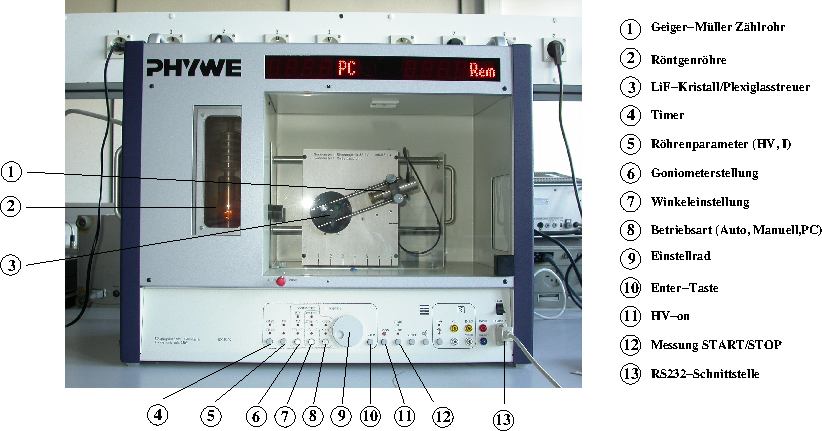
\includegraphics[width=0.5\textwidth]{content/img/Abb_2.pdf}
        \caption{Der schematische Aufbau des Auges. \cite{versuchsanleitung}}
        \label{fig:augenmodell}
    \end{figure}

    Für die Messung mit der Ultraschallsonde wird Ultraschallgel verwendet,
    damit die Sonde leichter auf der Oberfläche des Auges bewegt werden kann.
    Es werden drei Peaks gemessen,
    die jeweils von der Iris, der Linse und der Retina verursacht werden,
    und die entsprechenden Laufzeiten und Amplituden der Schallimpulse notiert.\\
    \\
    Nach Abschluss der Messungen müssen die Ultraschallsonde und die Proben
    mithilfe von weichen Tüchern und Wasser vorsichtig gereinigt werden.
